\appendix

% Changes the table and figure counting to A.1 style
\renewcommand\thefigure{\thechapter.\arabic{figure}}
\renewcommand\thetable{\thechapter.\arabic{table}}
\setcounter{figure}{0}
\setcounter{table}{0}

\chapter{PEMcoupling examples}\label{app:pemcoupling}

This appendix presents examples of files produced by the \pemcoupling package to give readers some guidance on interpreting the outputs.
Each injection is given its own directory in which results are are saved and an HTML page is created with a table of links to the output files, sorted by channel name (Figure~\ref{fig:pemcoupling-html}).

\begin{figure}
  \centering
  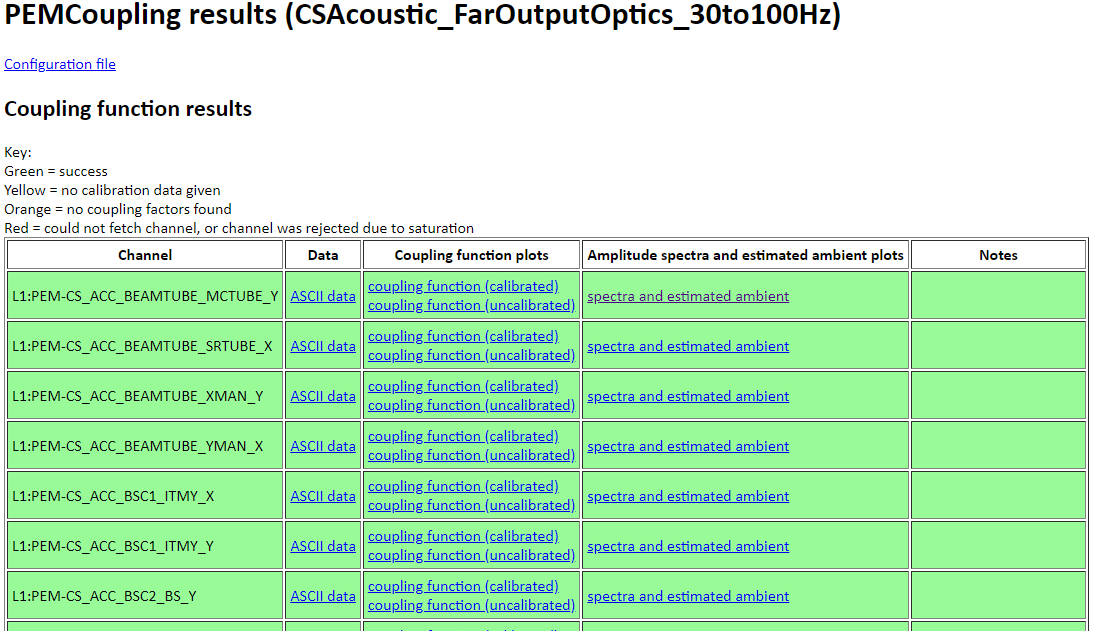
\includegraphics[width=0.8\textwidth]{figures/appendix/pemcoupling-html.png}
  \caption{HTML page for a single-injection coupling function run.}
  \label{fig:pemcoupling-html }
\end{figure}

There are two types of figures produced by \pemcoupling at the single-injection, single-sensor level: a coupling function plot and an estimated ambient plot.
Coupling function plots are produced in the physical, calibrated, sensor units (Figure~\ref{fig:pemcoupling-cf-physical}), as well as in raw counts (Figure~\ref{fig:pemcoupling-cf-raw}).
In the former case the units will look like [m/T] for magnetometers, while in the latter the units are [m/counts], regardless of sensor type.
Estimated ambients are always shown in calibrated units (Figure~\ref{fig:pemcoupling-cf-ambient}).
Each plot is annotated with information about the injection and analysis.
From left to right, top to bottom:
\begin{itemize}
  \item Name of the injection, as specified by the user.
  \item Timestamp of when the analysis was run.
  \item Number of Number of measurements and upper limits computed.
  \item UTC and GPS start time of the injection data.
  \item Number of FFT averages and frequency bin width.
  \item UTC and GPS start time of the background data.
\end{itemize}

Table~\ref{tab:pemcoupling-format} summarizes the contents of the output ASCII data output file.
The data will be preceded by a commented line (starting with a \code{\#} character) denoting the comb fundamental frequency if the injection was a comb injection, e.g. \code{\#combfreq:7.10}.

\begin{figure}
  \centering
  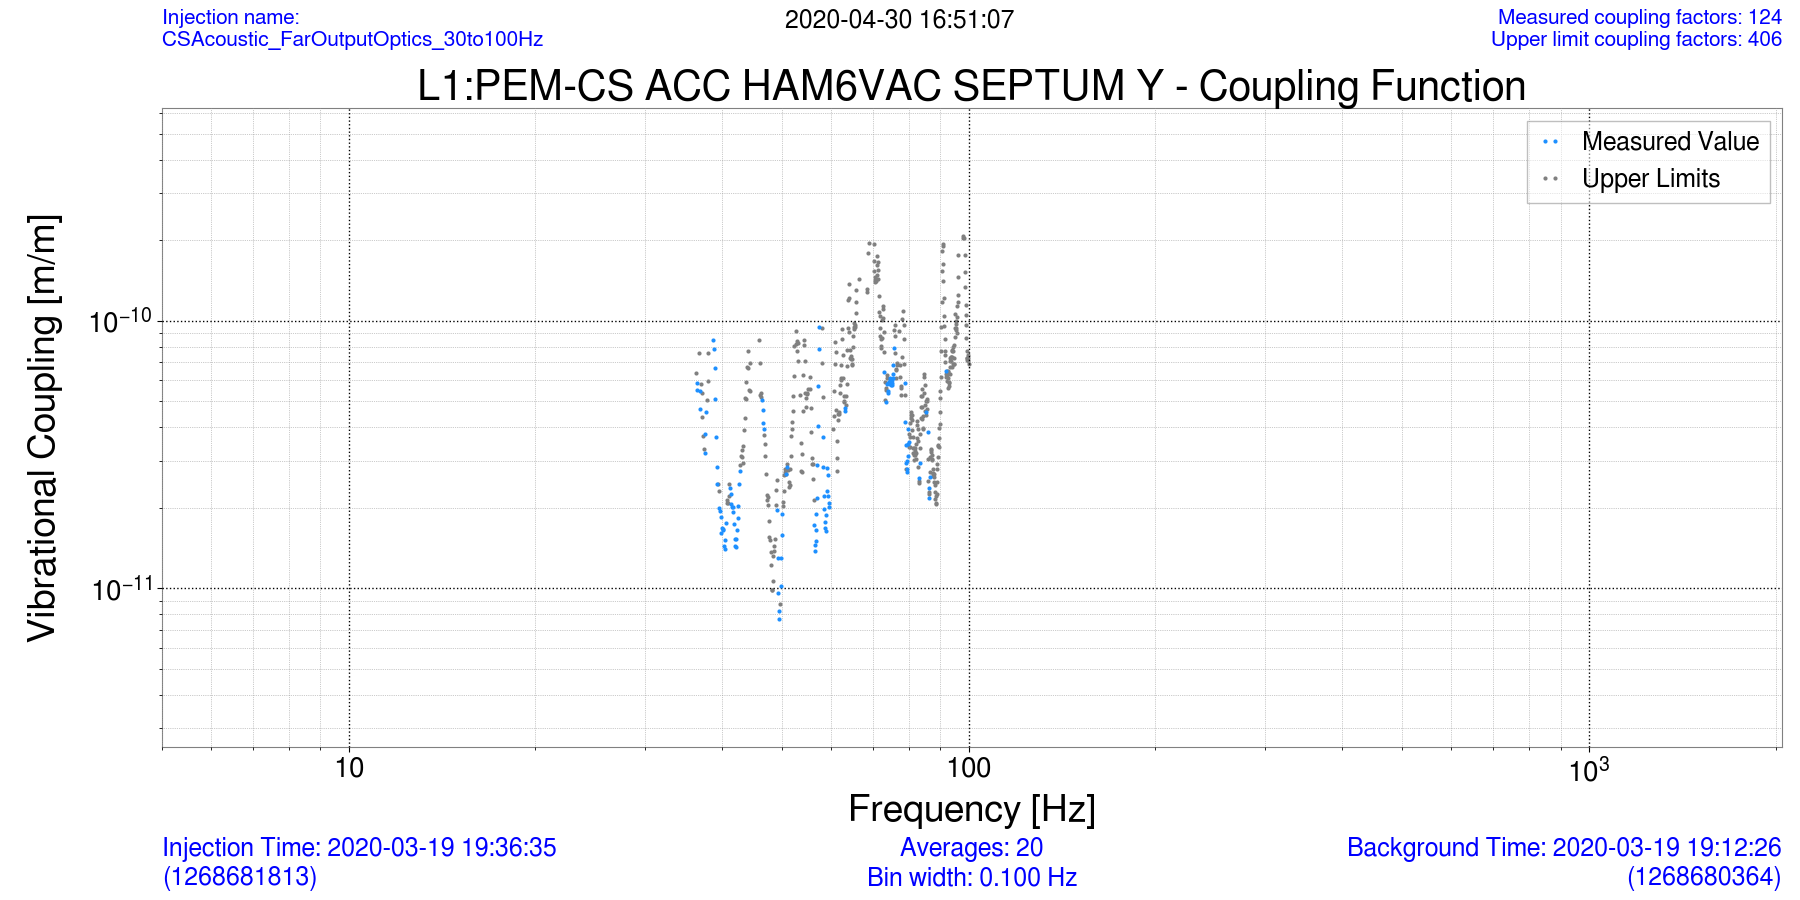
\includegraphics[width=0.9\textwidth]{figures/appendix/pemcoupling-cf-physical.png}
  \caption{Coupling function in physical units for the Y-axis HAM 5/6 septum accelerometer from a broadband acoustic injection.}
  \label{fig:pemcoupling-cf-physical}
\end{figure}

\begin{figure}
  \centering
  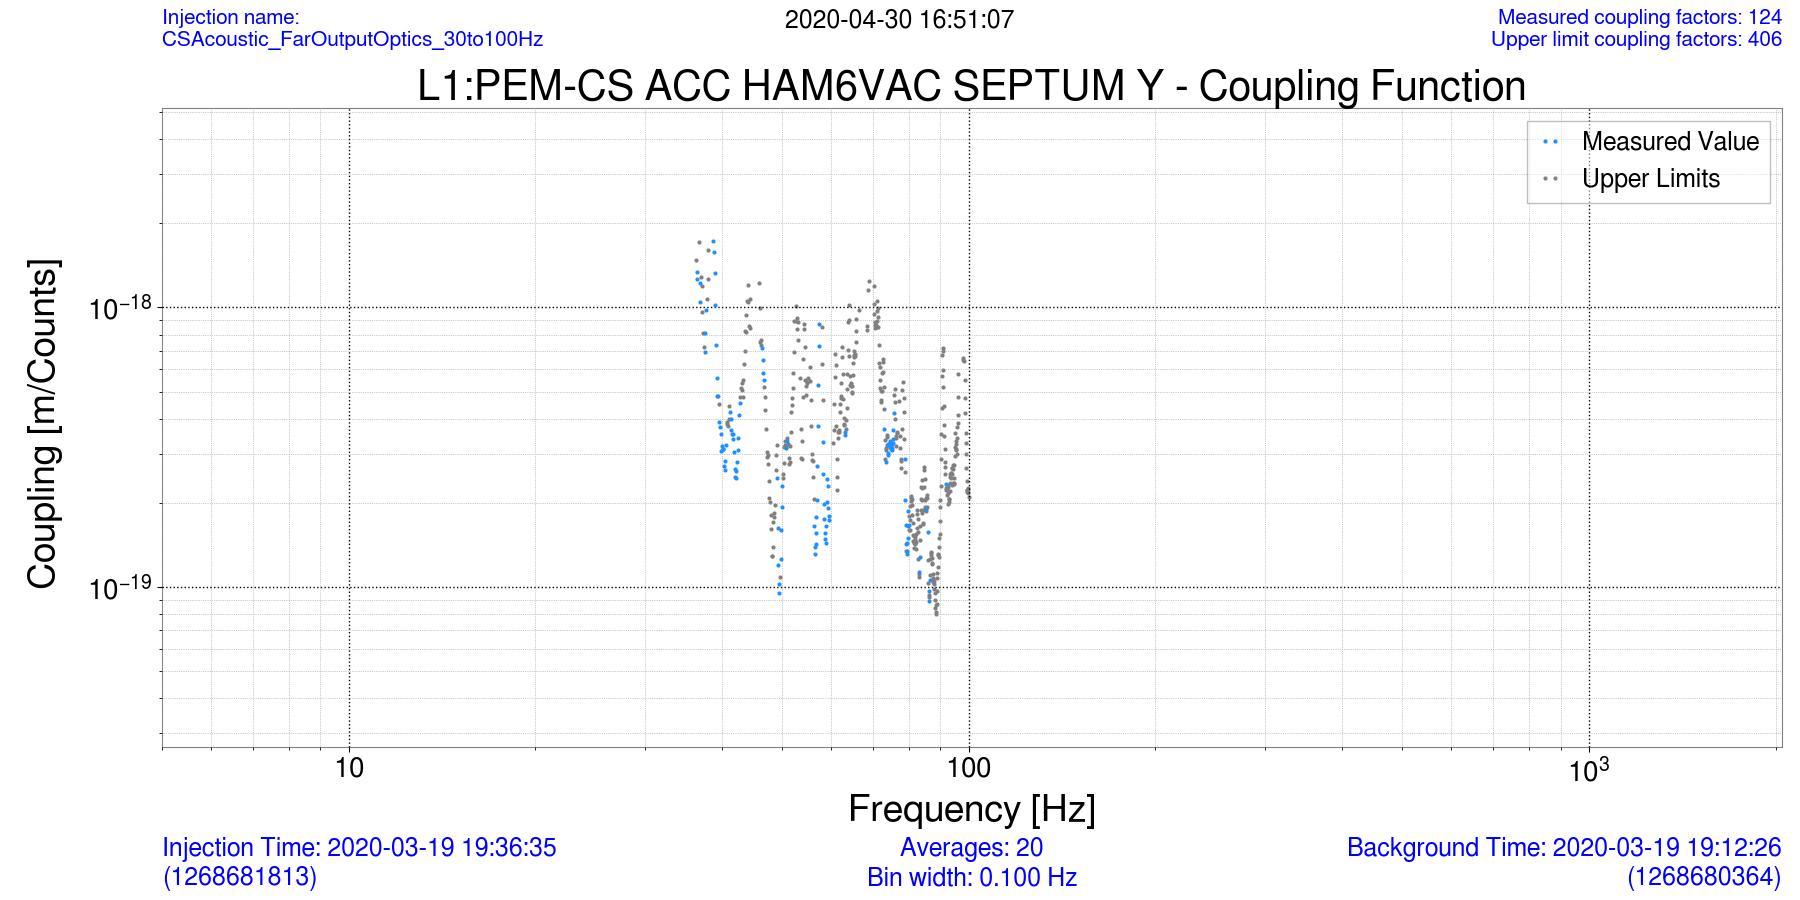
\includegraphics[width=0.9\textwidth]{figures/appendix/pemcoupling-cf-raw.png}
  \caption{Coupling function in ADC counts for the Y-axis HAM 5/6 septum accelerometer from a broadband acoustic injection.}
  \label{fig:pemcoupling-cf-raw}
\end{figure}

\begin{figure}
  \centering
  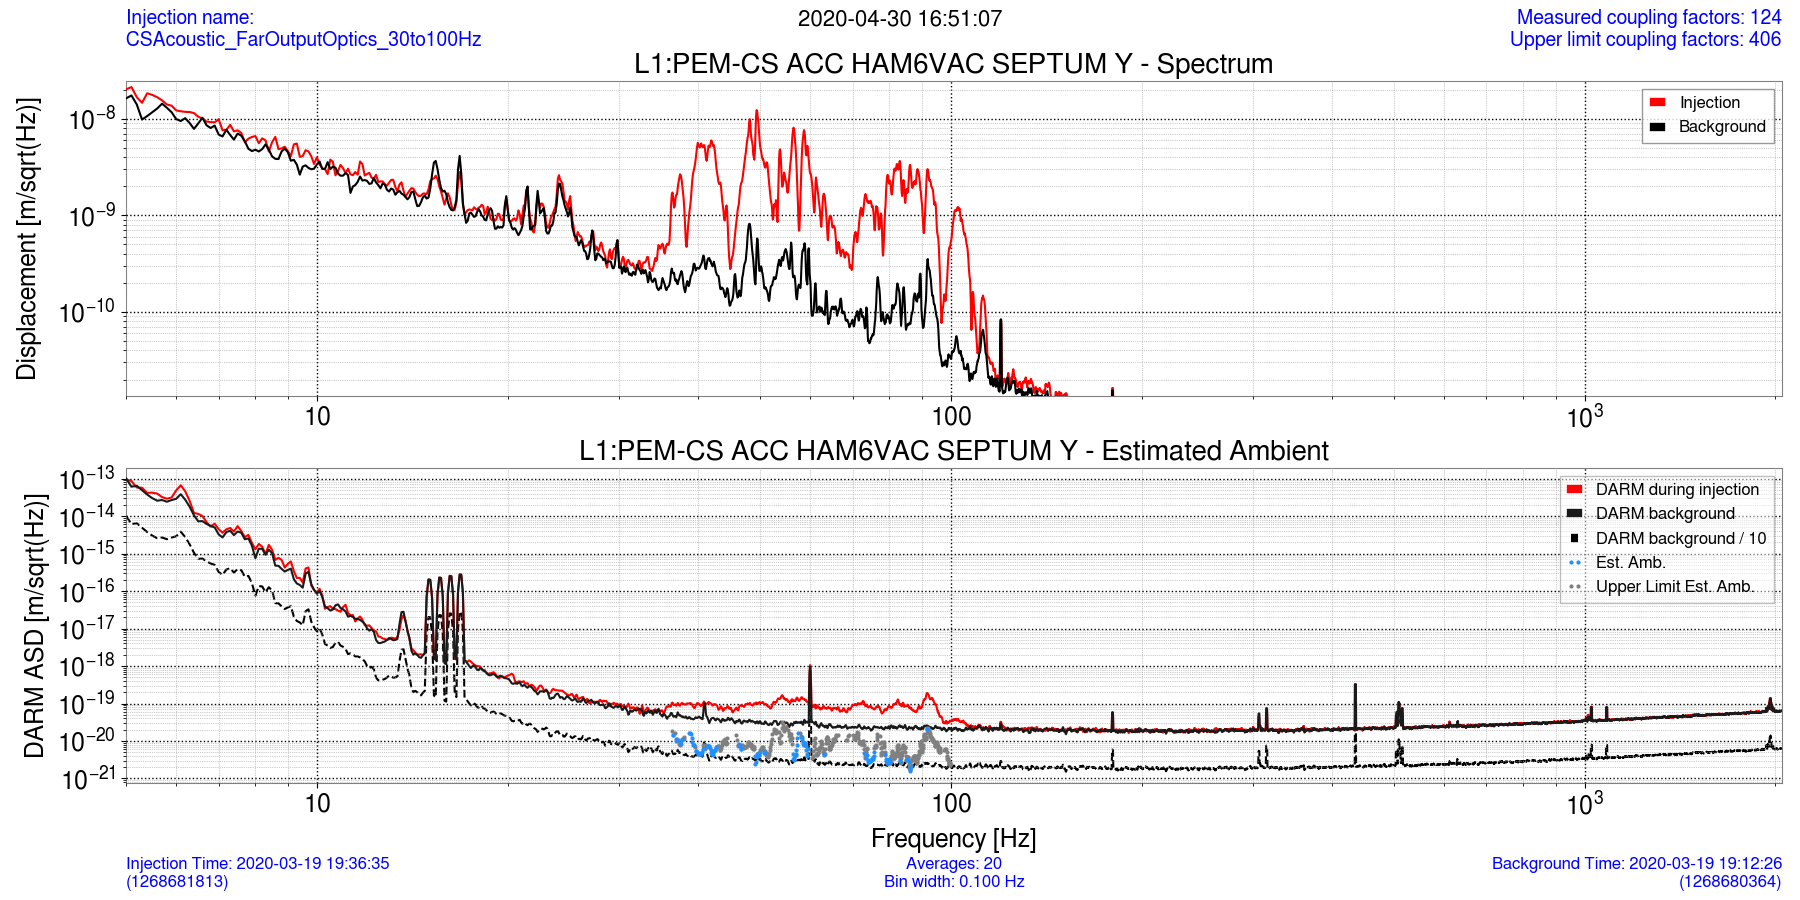
\includegraphics[width=0.9\textwidth]{figures/appendix/pemcoupling-cf-ambient.png}
  \caption{Estimated ambient for the Y-axis HAM 5/6 septum accelerometer from a broadband acoustic injection.}
  \label{fig:pemcoupling-cf-ambient}
\end{figure}

\begin{table}
	\renewcommand{\arraystretch}{1.5}
	\begin{tabular}{|ll|}
		\hline
		\multicolumn{1}{|l}{\textbf{column}} & \multicolumn{1}{l|}{\textbf{description}}\\ \hline
		\code{frequency}      & bin center frequency {[}Hz{]}\\
		\code{factor}         & coupling factor in {[}m/calibrated sensor unit{]}\\
		\code{factor\_counts} & coupling factor in {[}m/ADC count{]}\\
		\code{flag}           & ``Measured", ``Upper Limit", ``Thresholds not met", or ``No data"\\
		\code{sensINJ}        & sensor amplitude at injection time {[}calibrated sensor unit$/\rthz${]}\\
		\code{sensBG}         & sensor amplitude at background time {[}calibrated sensor unit$/\rthz${]}\\
		\code{darmINJ}        & \ac{GW} channel amplitude at injection time $[\meter/\rthz]$\\
		\code{darmBG}         & \ac{GW} channel amplitude at background time $[\meter/\rthz]$\\ \hline
	\end{tabular}
	\caption{Column descriptions for the single-injection coupling function output of the \pemcoupling package.}
  \label{tab:pemcoupling-format}
\end{table}

Composite coupling function output files are saved to another directory, by default named \code{CompositeCouplingFunctions}.
These figures follow the same organization: a physical coupling function (with colors representing different injections, Figure~\ref{fig:pemcoupling-ccf-physical}), a raw coupling function (Figure~\ref{fig:pemcoupling-ccf-raw}), and an estimated ambient. (Figure~\ref{fig:pemcoupling-ccf-ambient}).
The raw-counts composite coupling function does not distinguish injections as it is only used to make noise projections, such as by \code{pemcheck}, as opposed to identify noise sources.

\begin{figure}
  \centering
  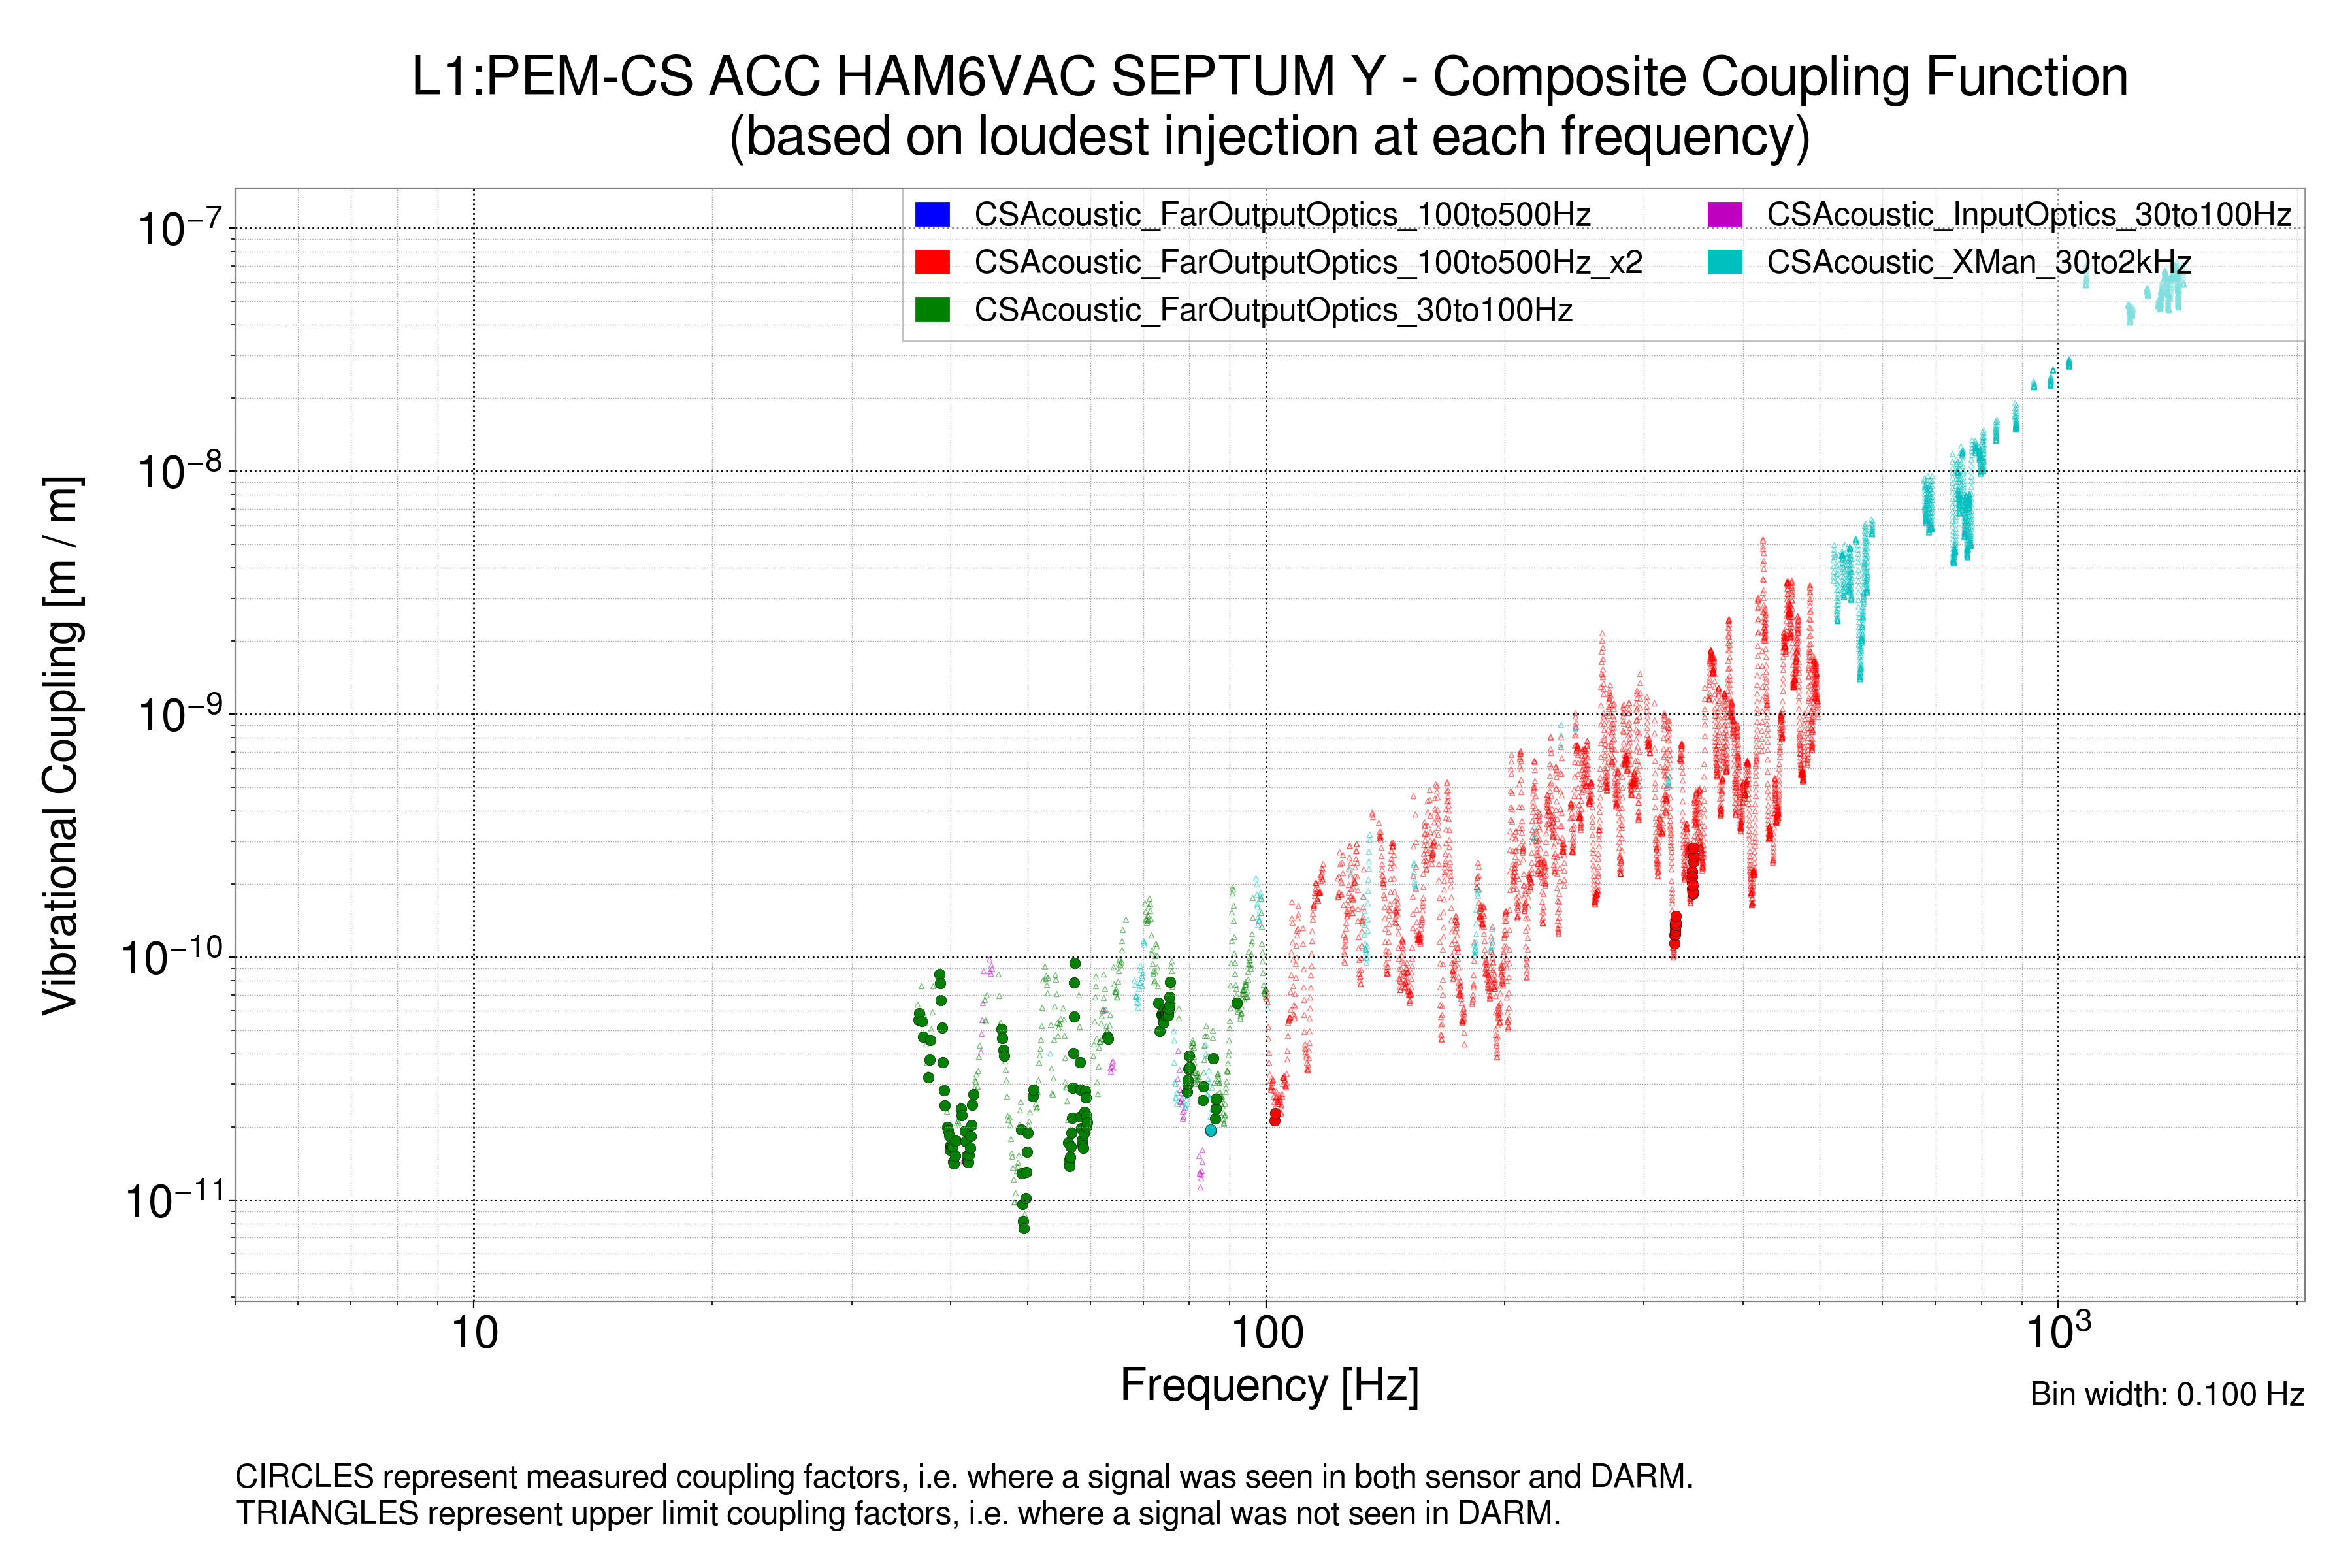
\includegraphics[width=0.9\textwidth]{figures/appendix/pemcoupling-ccf-physical.png}
  \caption{Composite coupling function in physical units for the Y-axis HAM 5/6 septum accelerometer.}
  \label{fig:pemcoupling-ccf-physical}
\end{figure}

\begin{figure}
  \centering
  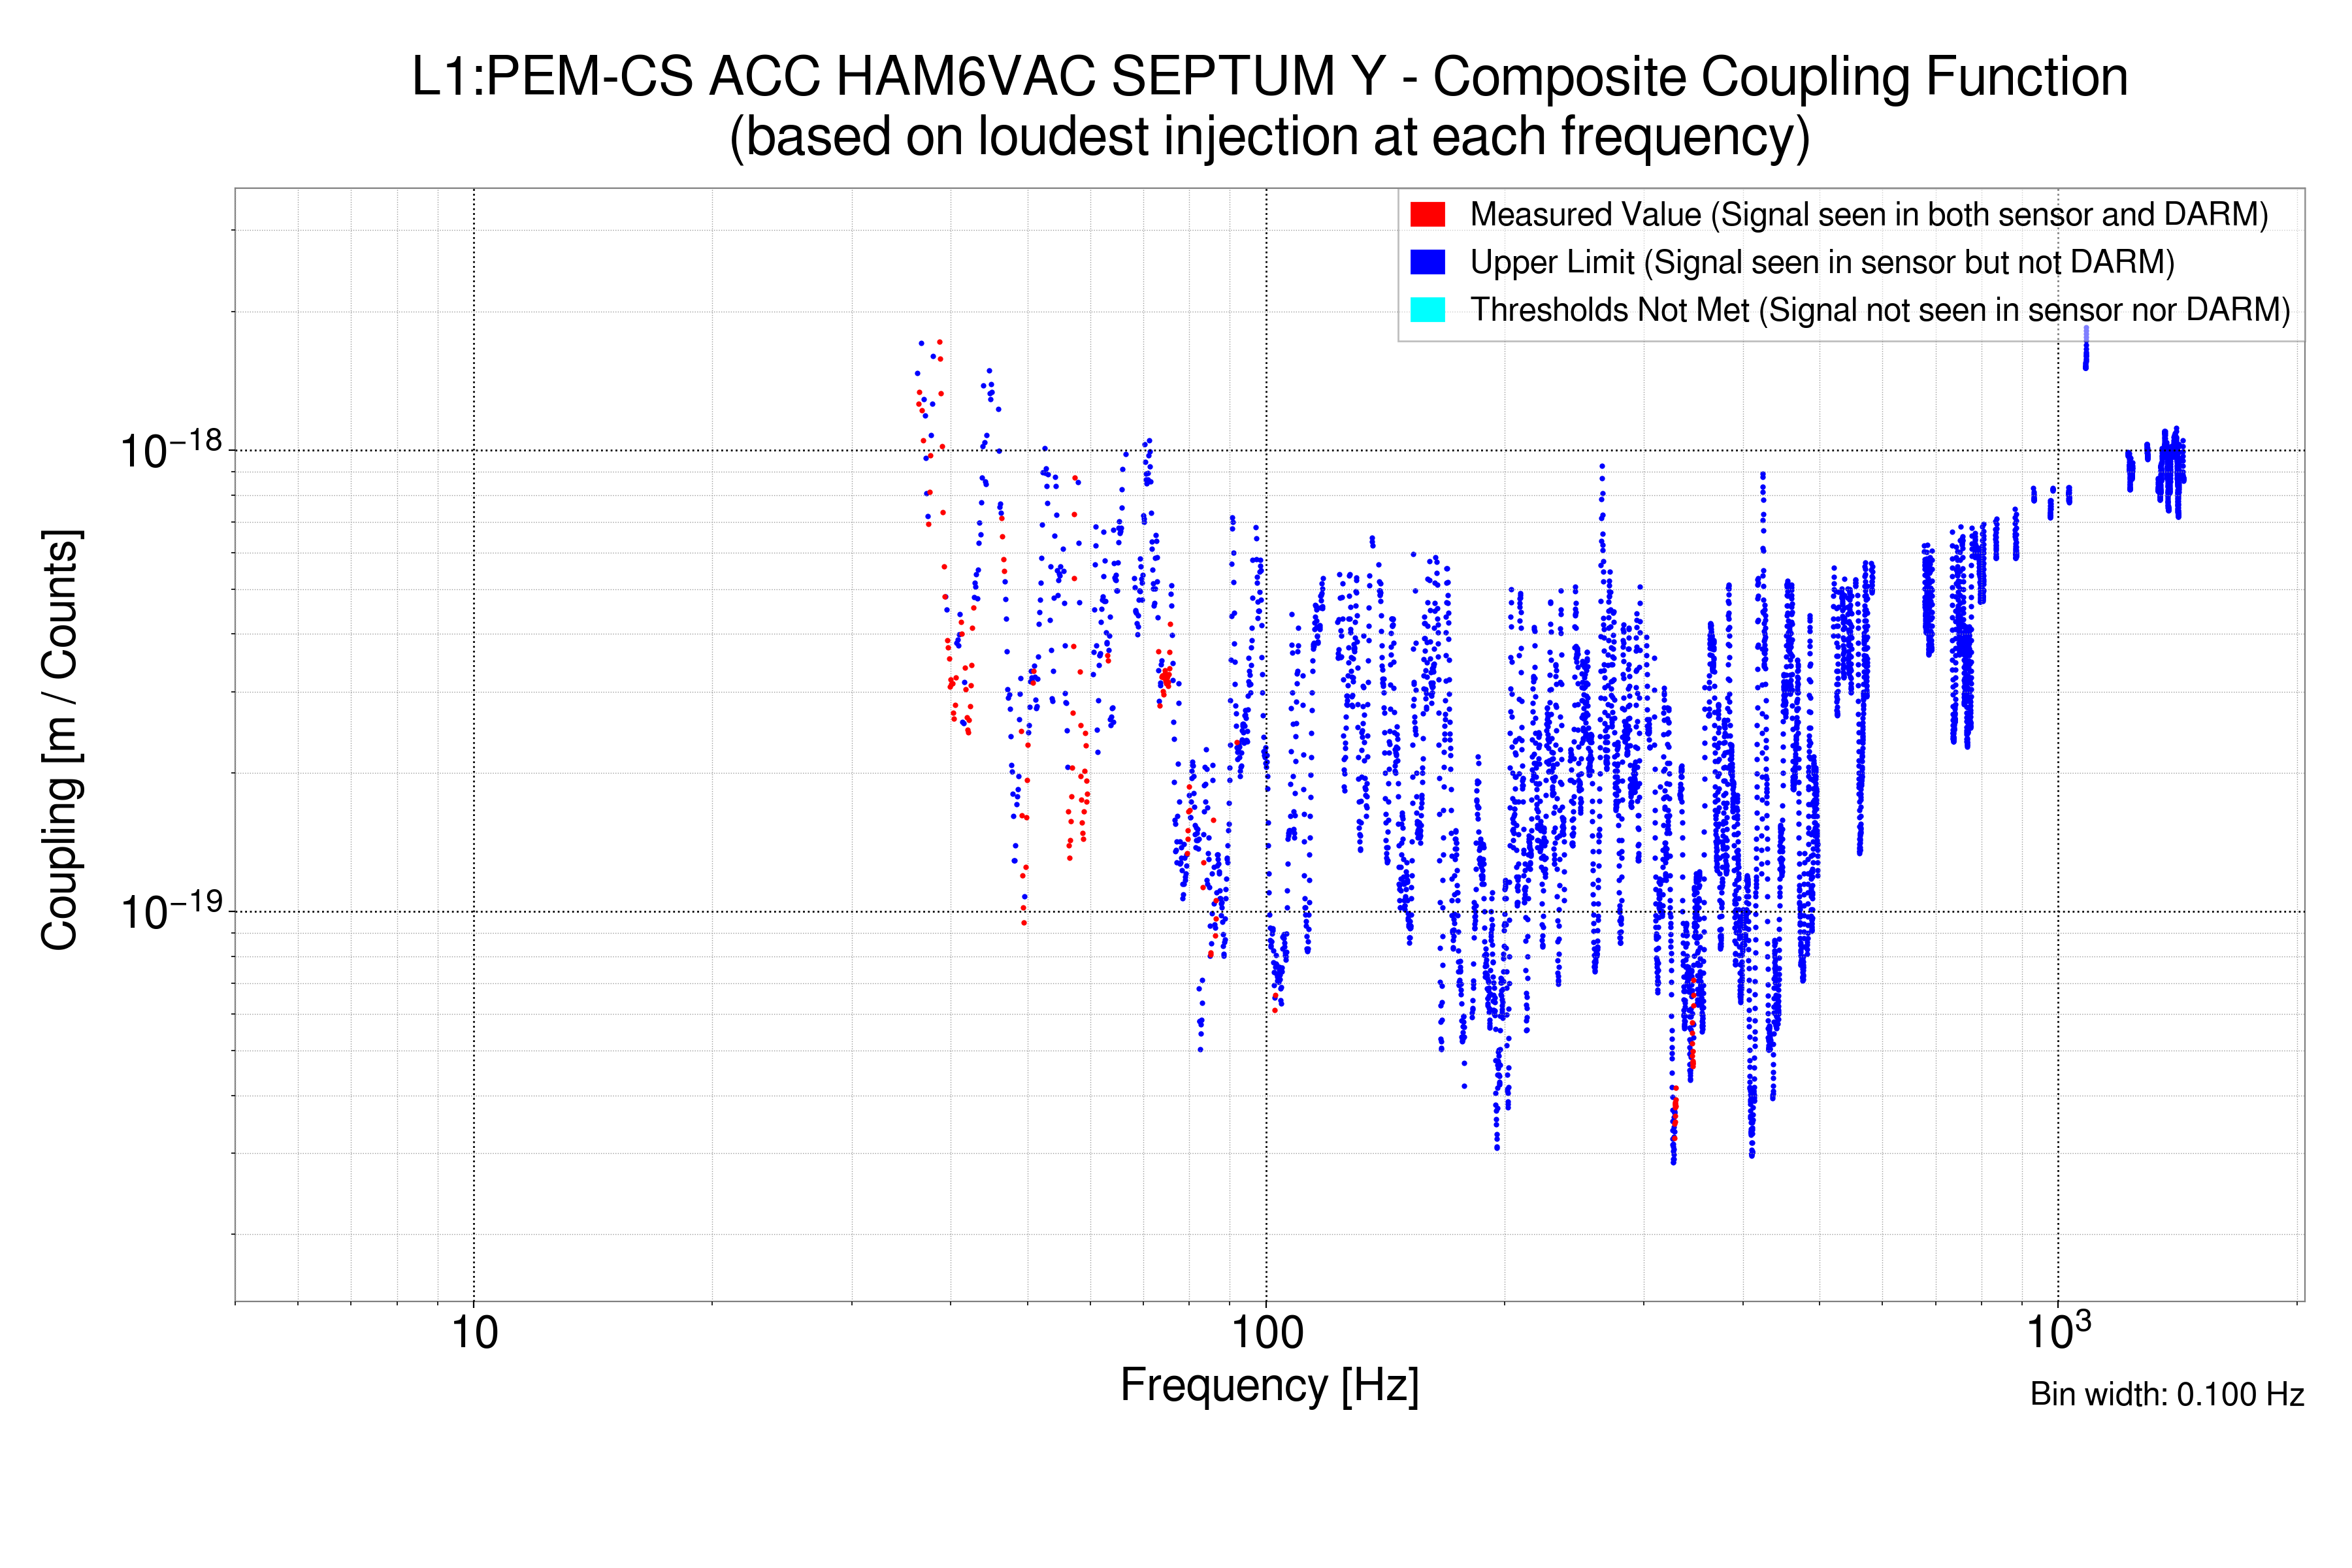
\includegraphics[width=0.9\textwidth]{figures/appendix/pemcoupling-ccf-raw.png}
  \caption{Composite coupling function in physical units for the Y-axis HAM 5/6 septum accelerometer.}
  \label{fig:pemcoupling-ccf-raw}
\end{figure}

\begin{figure}
  \centering
  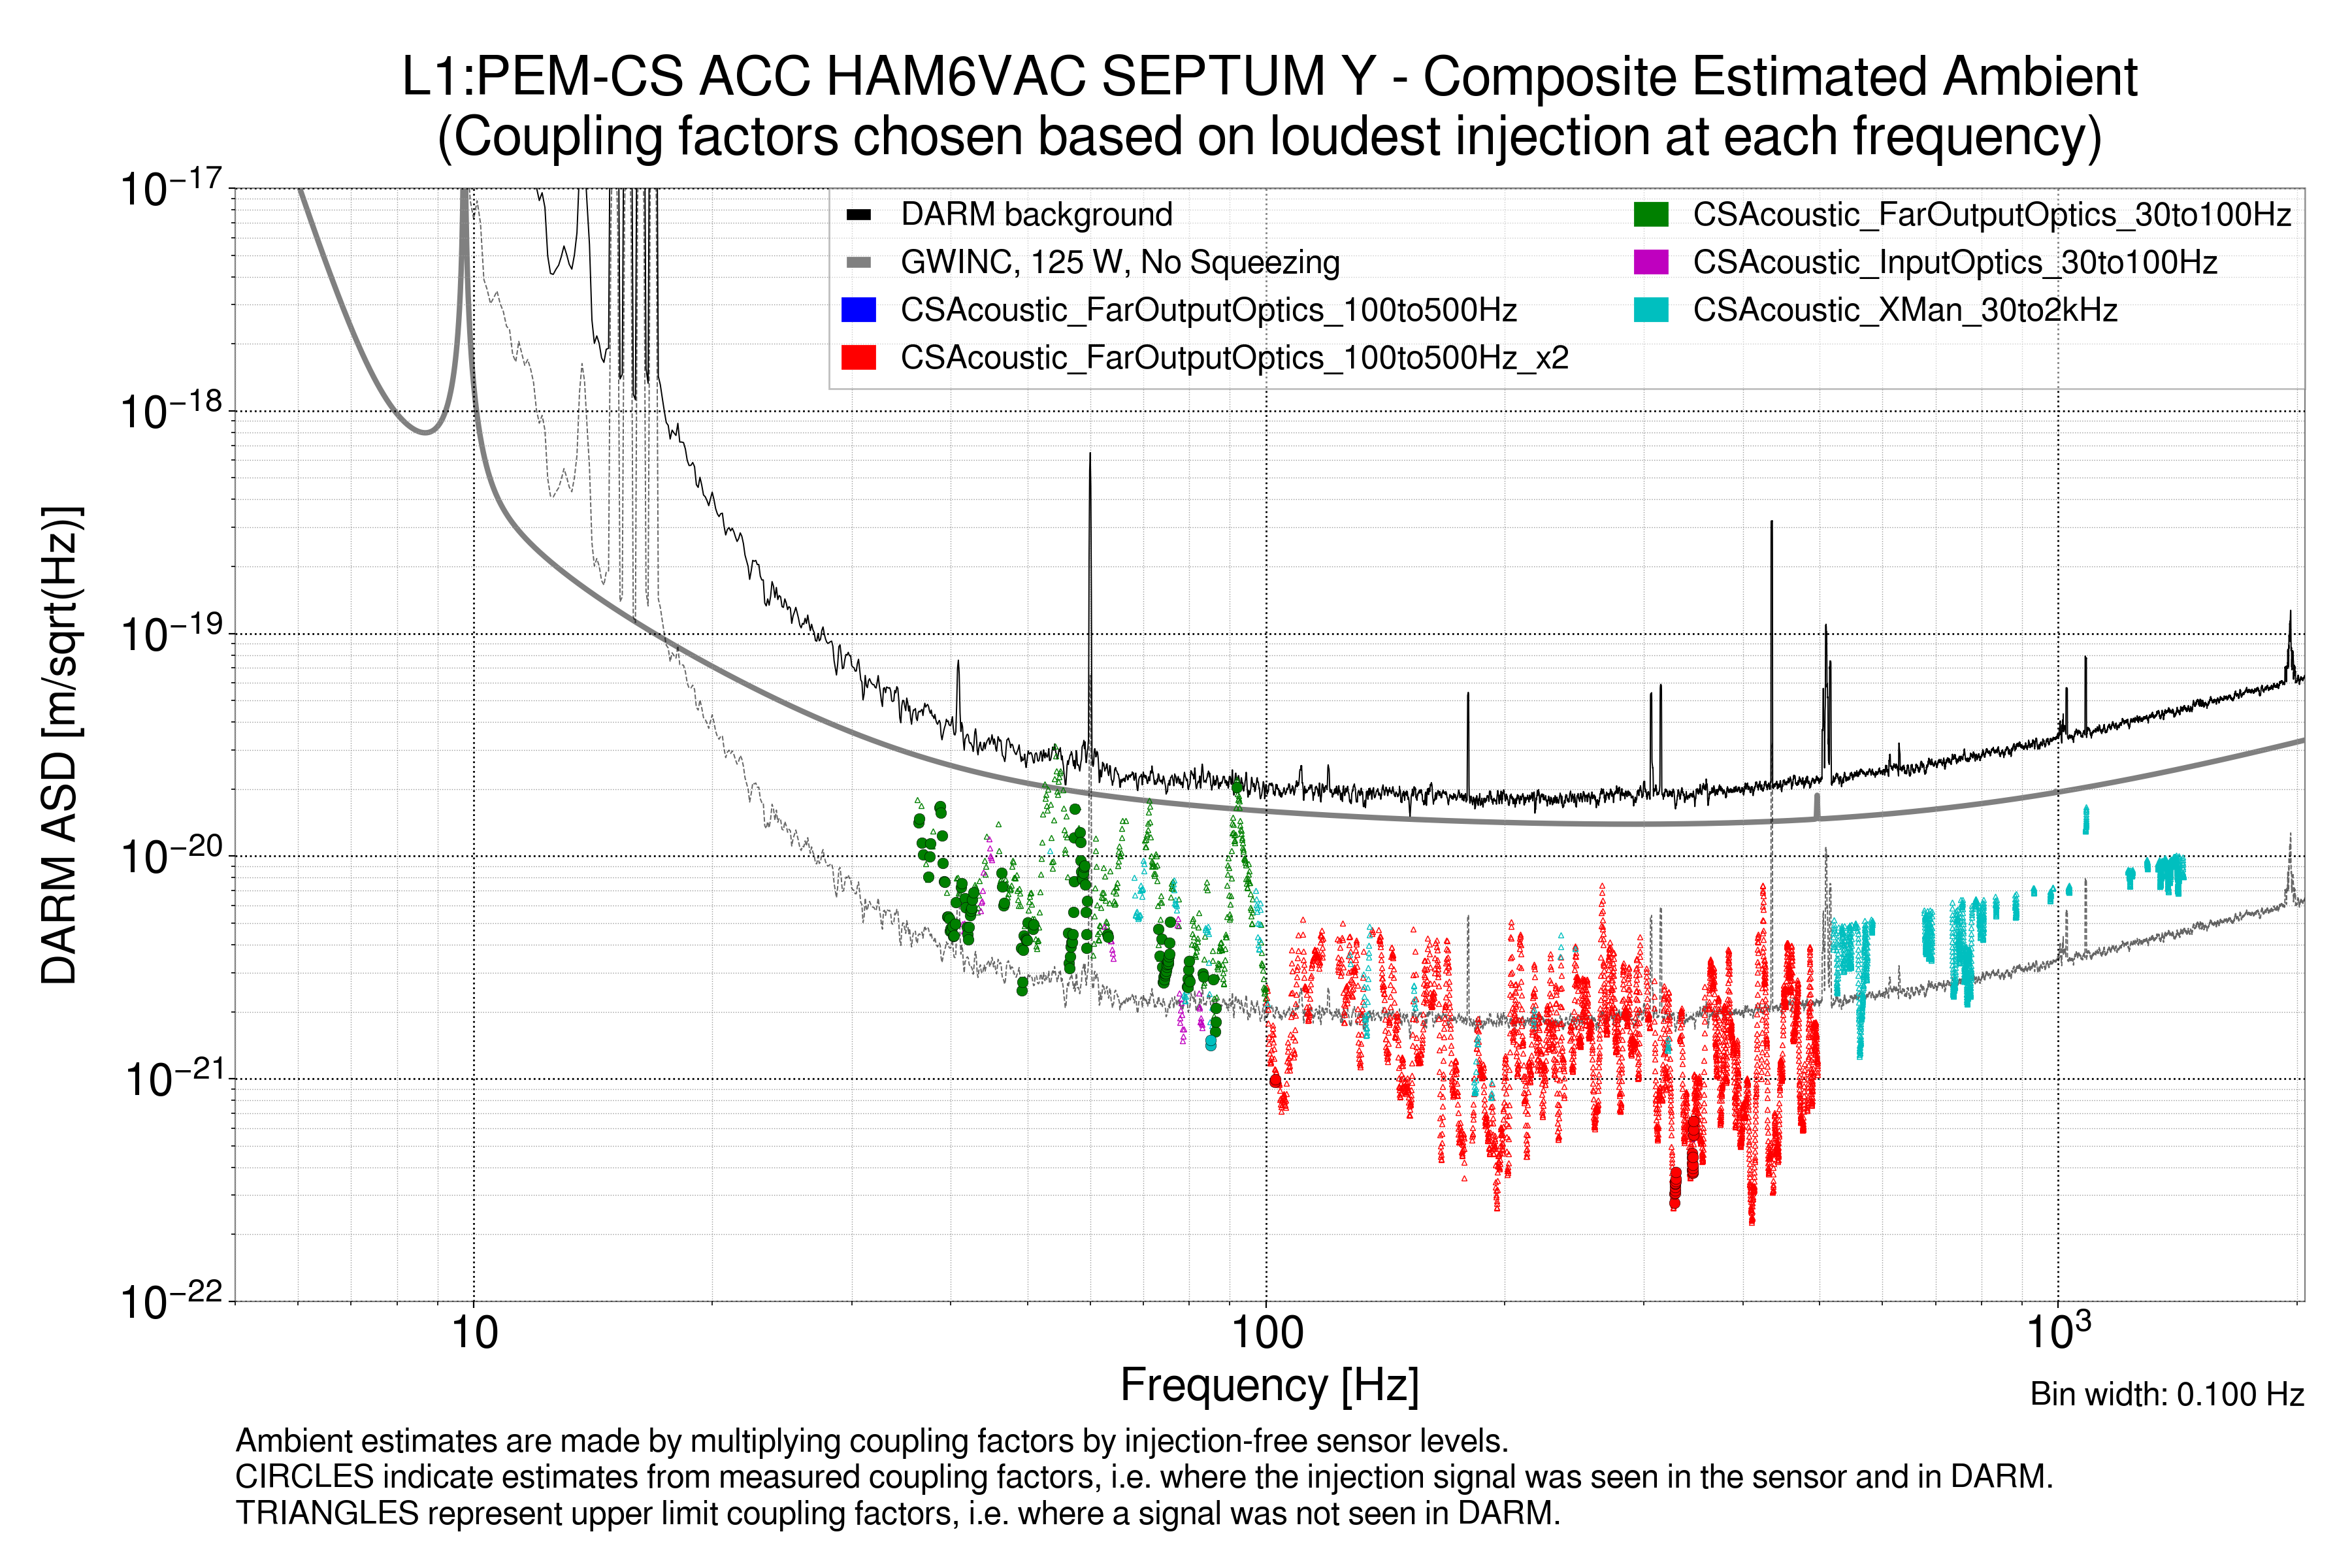
\includegraphics[width=0.9\textwidth]{figures/appendix/pemcoupling-ccf-ambient.png}
  \caption{Estimated ambient for the Y-axis HAM 5/6 septum accelerometer.}
  \label{fig:pemcoupling-ccf-ambient}
\end{figure}

Last is an example of a site-wide estimated ambient (Figure~\ref{fig:pemcoupling-sitewide-ambient}) plot.

\begin{figure}
  \centering
  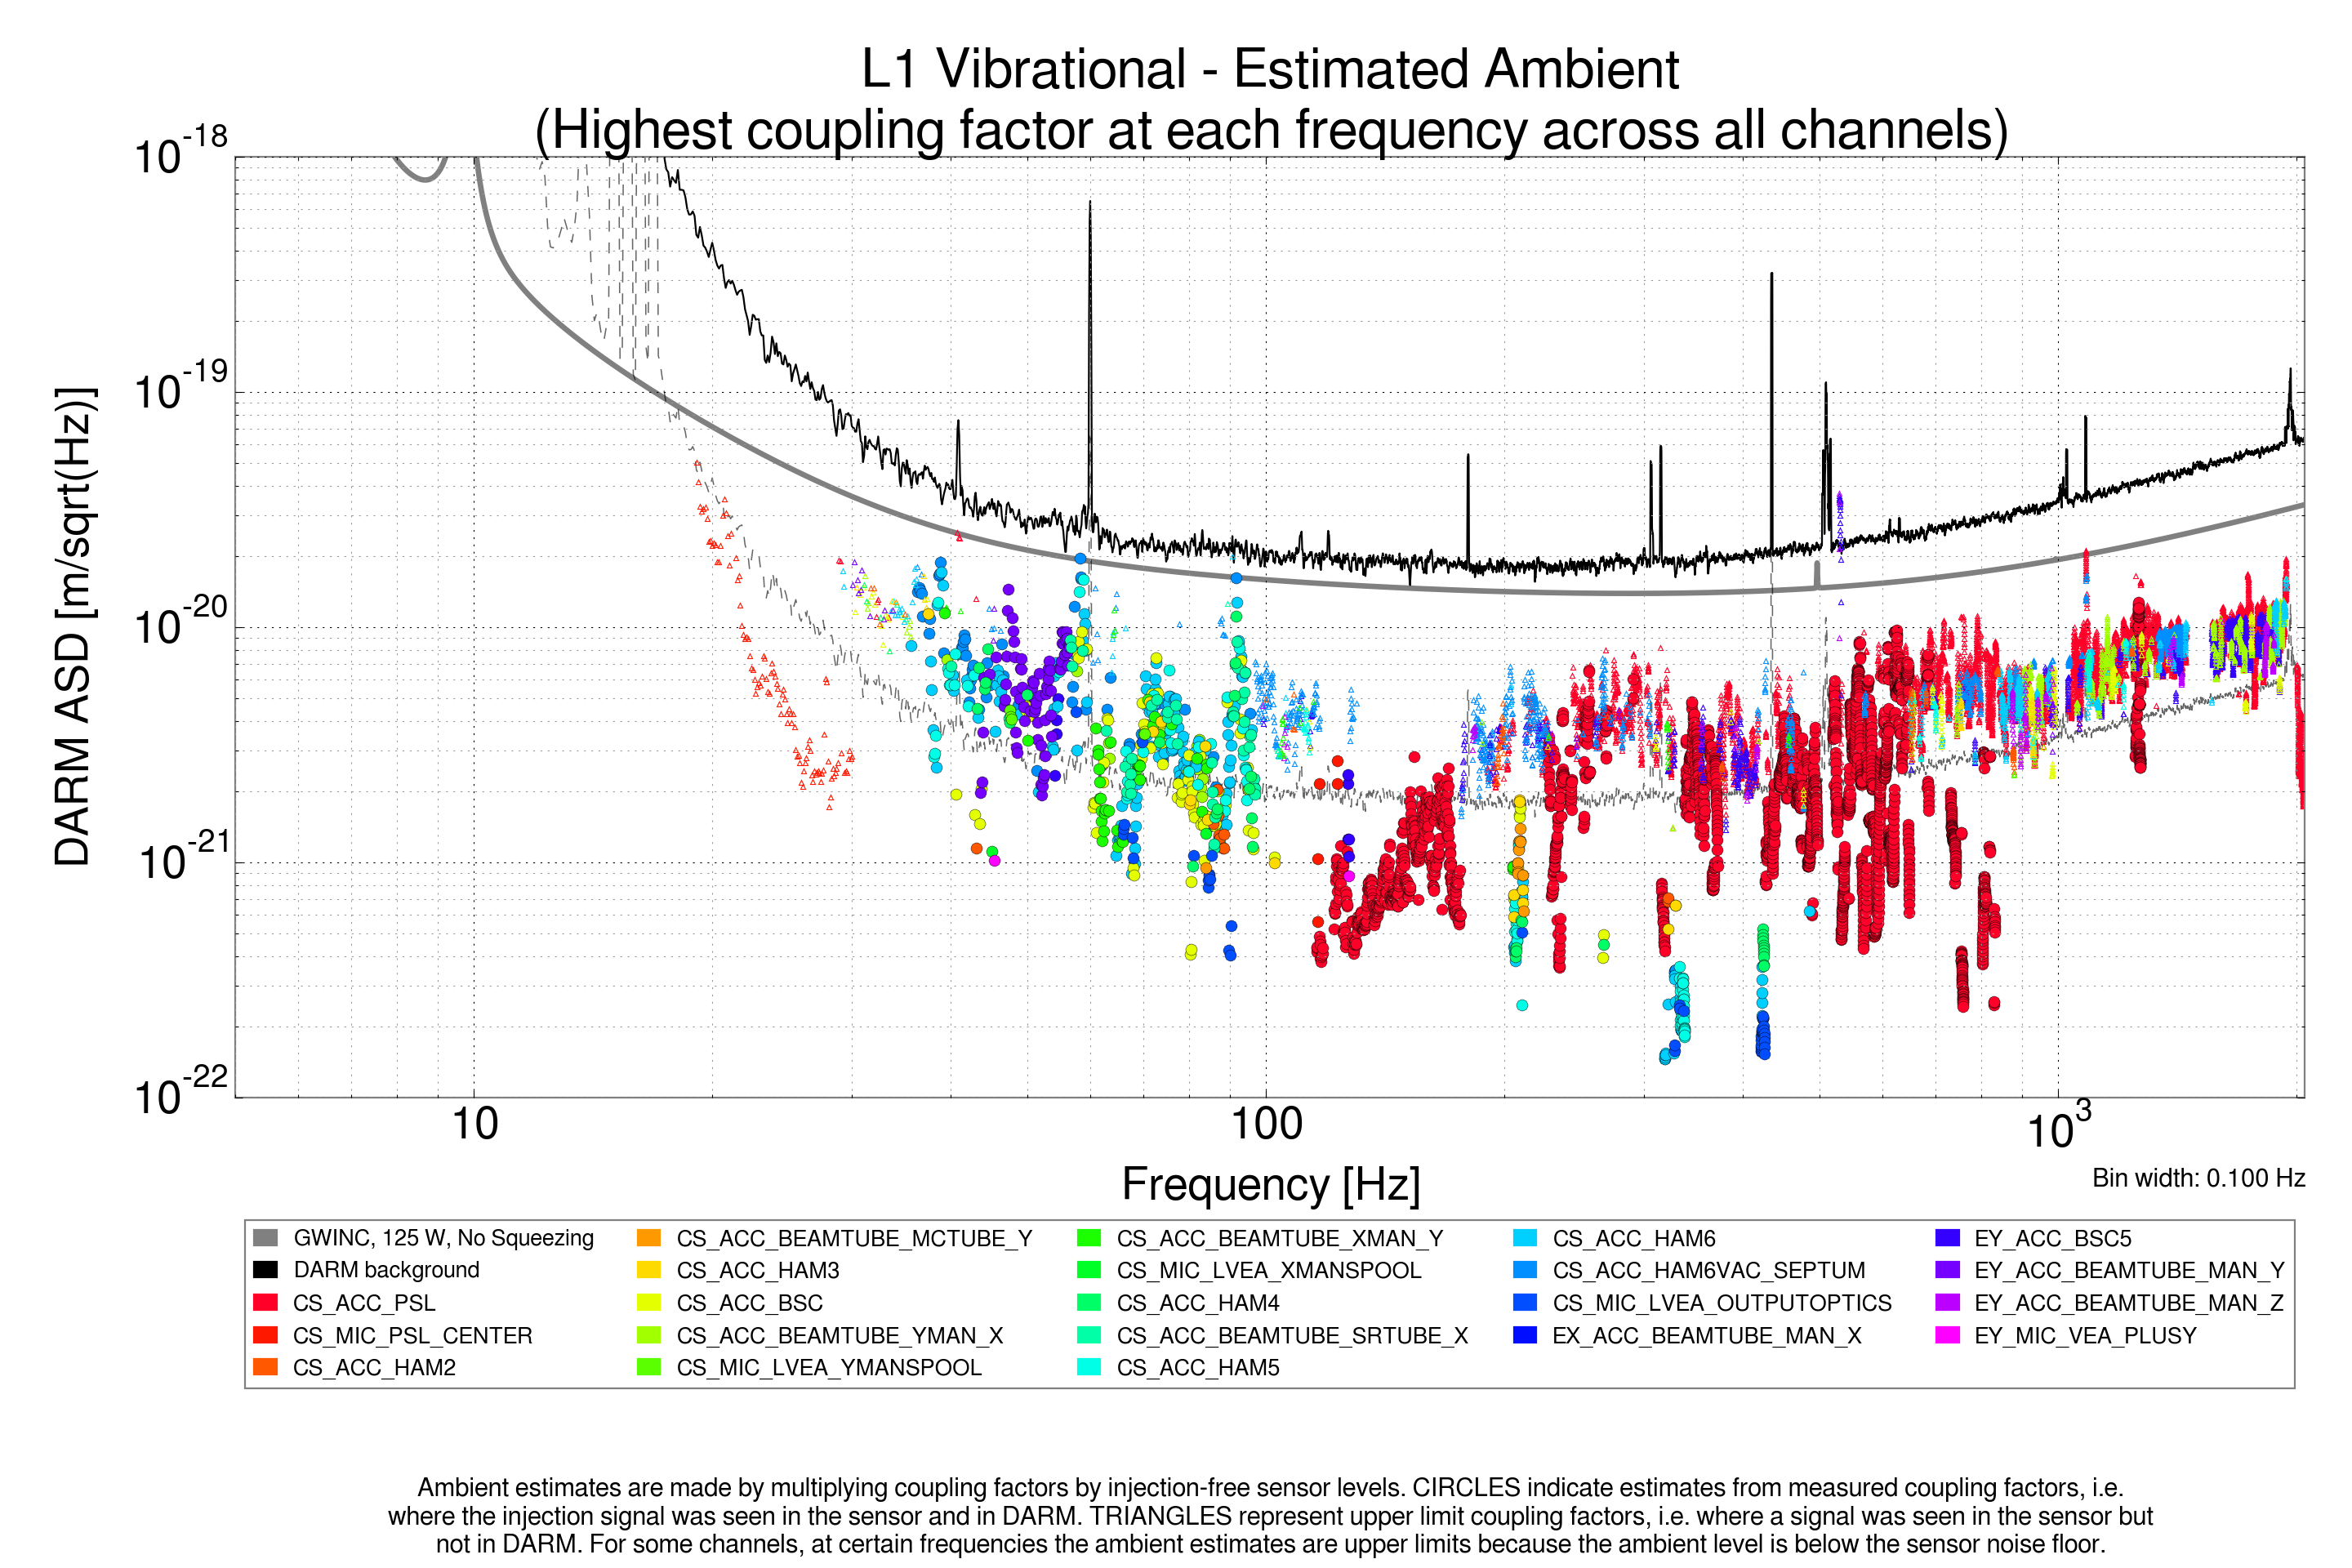
\includegraphics[width=0.9\textwidth]{figures/appendix/pemcoupling-sitewide-ambient.png}
  \caption{Site-wide estimated ambient for all vibrational sensors at LLO.}
  \label{fig:pemcoupling-sitewide-ambient}
\end{figure}


% Restart counting to B.1, B.2...
\setcounter{figure}{0}
\setcounter{table}{0}

\chapter{PEMcheck examples}\label{app:pemcheck}

This appendix presents screenshots of \code{pemcheck} output pages tested on GW events and environmental noise transients.

\begin{figure}
  \centering
  % \includegraphics[width=\textwidth]{/path/to/figure}
  \caption{Example report page produced by \protect\code{pemcheck} for a long duration GW event.}
  \label{fig:pemcheck-GW190510g}
\end{figure}
